\begin{figure}[!h]
\centering
\resizebox{0.85\textwidth}{!}{%
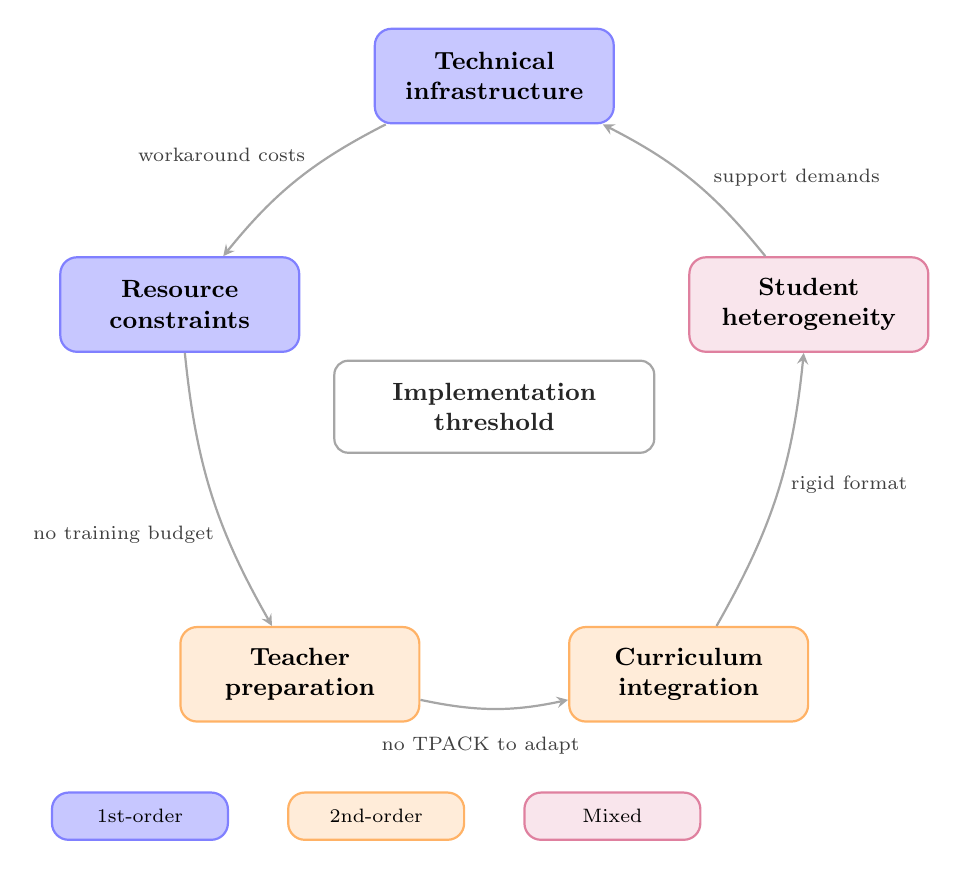
\begin{tikzpicture}[
  firstorder/.style={rectangle, rounded corners=6pt, draw=blue!50, fill=blue!22,
    text width=2.8cm, minimum height=1.2cm, align=center, font=\small\bfseries,
    line width=0.8pt},
  secondorder/.style={rectangle, rounded corners=6pt, draw=orange!60, fill=orange!15,
    text width=2.8cm, minimum height=1.2cm, align=center, font=\small\bfseries,
    line width=0.8pt},
  mixedorder/.style={rectangle, rounded corners=6pt, draw=purple!50,
    fill=purple!10, text width=2.8cm, minimum height=1.2cm, align=center,
    font=\small\bfseries, line width=0.8pt},
  arr/.style={->, >=stealth, thick, draw=gray!70},
  lbl/.style={font=\scriptsize, text=gray!50!black, fill=white, inner sep=2pt},
]

% Pentagon layout (72-degree spacing)
\node[firstorder] (tech) at (90:4.2) {Technical\\infrastructure};
\node[firstorder] (res) at (162:4.2) {Resource\\constraints};
\node[secondorder] (teach) at (234:4.2) {Teacher\\preparation};
\node[secondorder] (curr) at (306:4.2) {Curriculum\\integration};
\node[mixedorder] (stud) at (18:4.2) {Student\\heterogeneity};

% Directed arrows with labels (clockwise cycle)
\draw[arr] (tech) to[bend right=12]
  node[lbl, pos=0.4, anchor=south east] {workaround costs}
  (res);
\draw[arr] (res) to[bend right=12]
  node[lbl, pos=0.6, anchor=north east] {no training budget}
  (teach);
\draw[arr] (teach) to[bend right=12]
  node[lbl, pos=0.4, anchor=north, yshift=-8pt] {no TPACK to adapt}
  (curr);
\draw[arr] (curr) to[bend right=12]
  node[lbl, pos=0.6, anchor=north west] {rigid format}
  (stud);
\draw[arr] (stud) to[bend right=12]
  node[lbl, pos=0.4, anchor=south west] {support demands}
  (tech);

% Central annotation
\node[draw=gray!70, fill=white, rounded corners=5pt,
  font=\small\bfseries, text=gray!30!black, inner sep=8pt,
  line width=0.8pt, text width=3.5cm, align=center]
  at (0, 0)
  {Implementation\\threshold};

% Legend
\node[firstorder, minimum height=0.6cm, text width=2cm, font=\scriptsize]
  at (-4.5, -5.2) {1st-order};
\node[secondorder, minimum height=0.6cm, text width=2cm, font=\scriptsize]
  at (-1.5, -5.2) {2nd-order};
\node[mixedorder, minimum height=0.6cm, text width=2cm, font=\scriptsize]
  at (1.5, -5.2) {Mixed};
\end{tikzpicture}%
}% end resizebox
\caption{Barrier interaction model: reinforcing cycles among five implementation barrier categories. The first-order/second-order distinction follows \citeauthor{Ertmer1999}~\cite{Ertmer1999}: first-order barriers (blue) involve external resources and infrastructure; second-order barriers (orange) involve knowledge, beliefs, and institutional culture; student heterogeneity (purple) crosses both orders. The central ``implementation threshold'' denotes the minimum resource--training--support level below which gamification cannot succeed regardless of design quality.}
\label{fig:barrier-interaction-model}
\end{figure}
